\documentclass{tufte-book}

\usepackage{tikz}
\usepackage{amsmath,amsthm,amssymb}
\usepackage{esint}
\usepackage{geometry}
\usepackage{setspace}
\usepackage{graphicx}
\usepackage{calc}
\graphicspath{ {./images/} }

\renewcommand{\b}{\mathbf}
\newcommand{\h}[1]{\mathbf{\hat{#1}}}
\def\r{{\mbox{$\resizebox{.09in}{.08in}{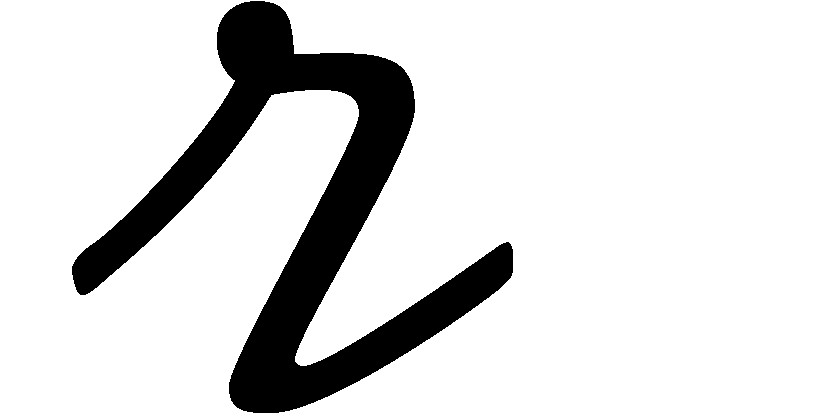
\includegraphics[trim= 1em 0 14em 0,clip]{ScriptR}}$}}}
\def\br{{\mbox{$\resizebox{.09in}{.08in}{
\includegraphics[trim= 1em 0 14em 0,clip]{BoldR}}$}}}

\setlength{\parindent}{0pt}

\title{Electromagnetism}
\author{Richard Robinson}

\begin{document}
\frontmatter
\maketitle
\tableofcontents
\mainmatter

\setlength{\parindent}{0pt}

%%%%%%%%%%%%%%%%%%%%%%%%%%%%%%%%%%%%%%%%%%%%%%%%%%%%%%%%%%%%%%

\chapter{Electrostatics}

\section{Electric Forces}
\textsc{In Electrodynamics}, there is typically a \textbf{source point} $\b r '$ where a charge is located and a \textbf{field point} $\b r$ where a field is calculated at. The \textbf{seperation vector} is defined as
\begin{equation}
  \br \equiv \b r - \b r ' \qquad \hat\br = \br/\r
\end{equation}
The force acting on a charge is given by \textbf{Coulomb's Law}, \begin{equation}
  \b F = k \sum \frac{q_1q_2}{\r^2} \hat\br = \iiint d \b F
\end{equation}
%
\begin{marginfigure}
  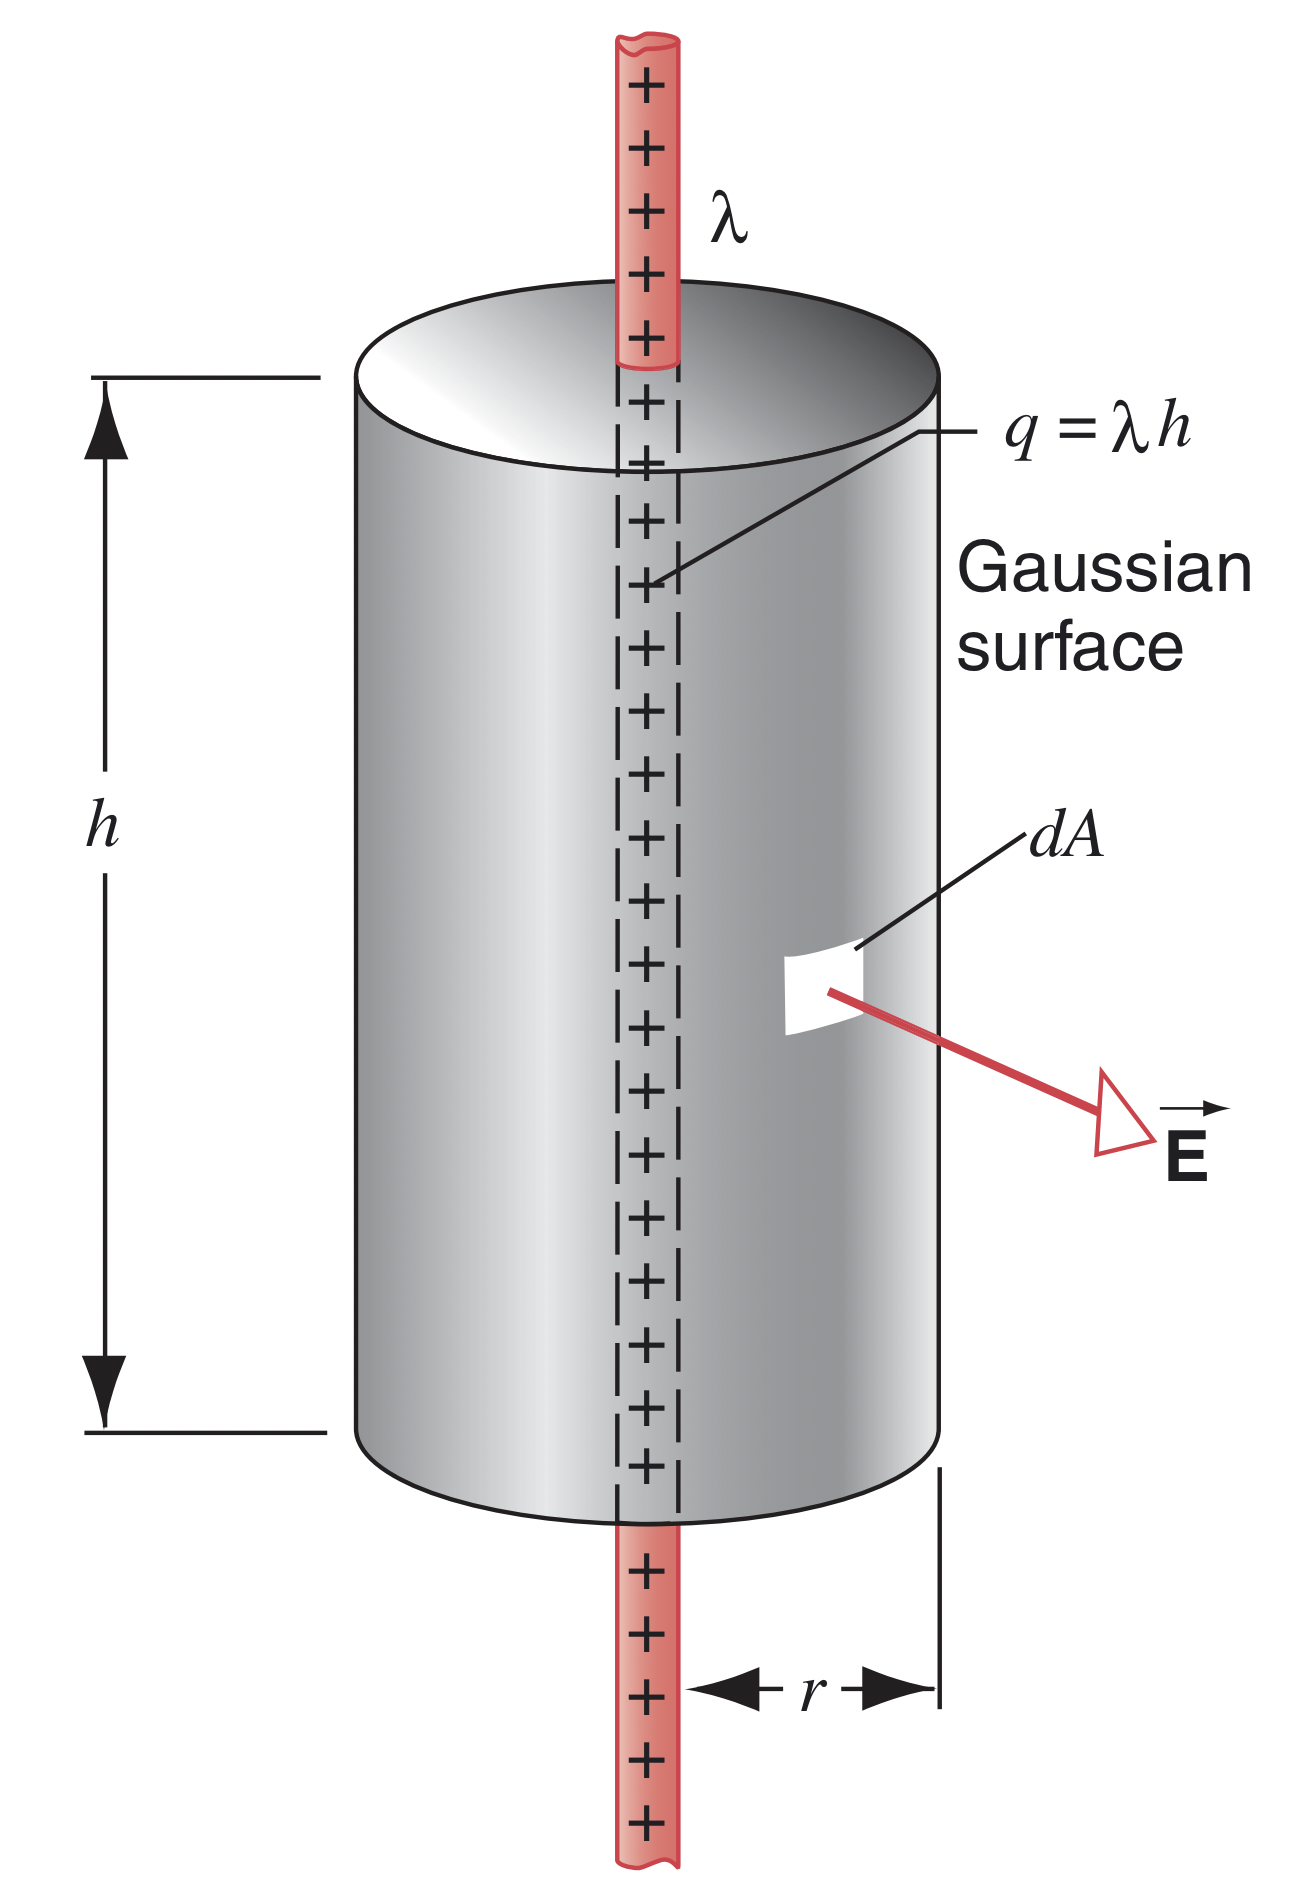
\includegraphics[scale=0.15]{field}
  \caption{A Gaussian surface as a cylinder.}
\end{marginfigure}
%
The \textbf{electric field} exerted on a positive test charge $+q_0$ at a point is defined as \begin{equation}
  \b E = \frac{\b F}{q_0} = k \sum \frac{q}{\r^2} \hat\br
\end{equation}
\textbf{Field lines} point outwards from $+q$ and towards $-q$, and are parallel or tangential of an electric field. For a continuous charge distribution, \begin{equation}
  \b E = k \iiint \frac{dq}{\r^2} \hat\br = - \nabla V
\end{equation}
where \begin{equation}
  dq \sim \lambda \, d \ell \sim \sigma \, d A \sim \rho \, dV \sim \lambda R \, d \phi \sim \sigma 2 \pi w \, d w
\end{equation}
The \textbf{electric dipole} is a configuration of two equal and opposite charges $q$ separated by a distance $d$, in which the electric dipole moment $p = qd$ in the direction towards $+q$. If a dipole is in an external field, the torque is \begin{equation}
  \b \tau = \b p \times \b E
\end{equation}
%
\begin{marginfigure}
  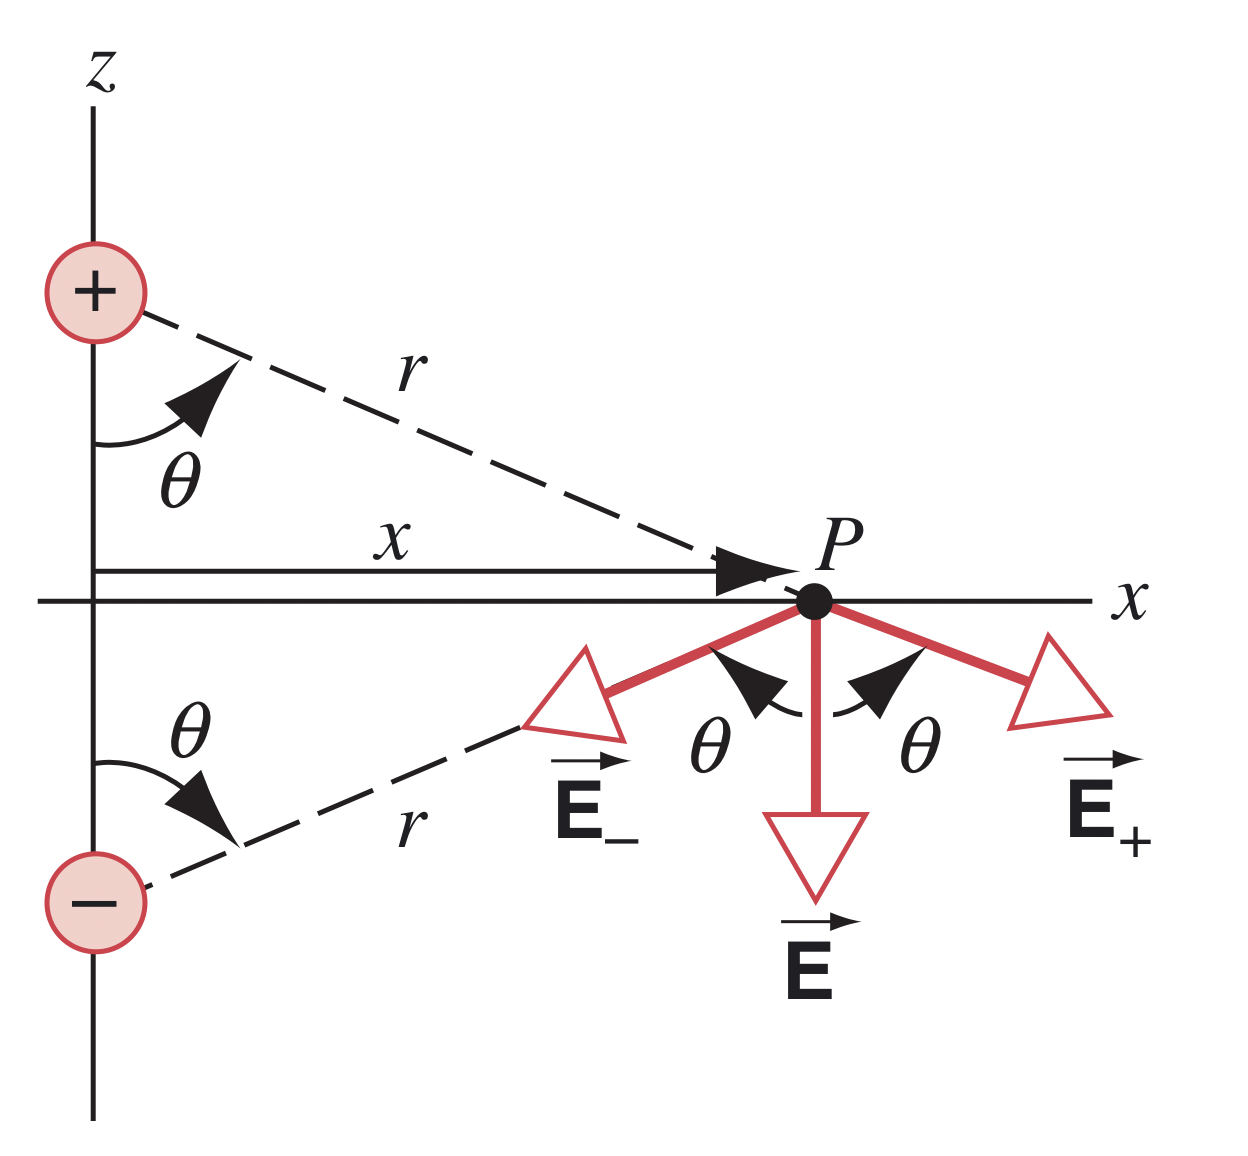
\includegraphics[width=0.8\textwidth]{dipole}
  \caption{The field at any is the vector sum of the charges.}
\end{marginfigure}
%
such that the work done by the field is \begin{equation}
  W = - \int_{\theta_0}^\theta \tau \; d \theta = pE(\Delta \cos \theta)
\end{equation}
Consequently, the potential energy is defined as \begin{equation}
  U = -pE \cos \theta = - \b p \cdot \b E
\end{equation}

\section{Potentials}
\textbf{Gauss' Law} states the electric \textbf{flux} through a field is \begin{equation}
  \Phi_E = \oiint \b E \cdot d \b A = \frac{q}{\varepsilon_0}
\end{equation}
%
\begin{marginfigure}
  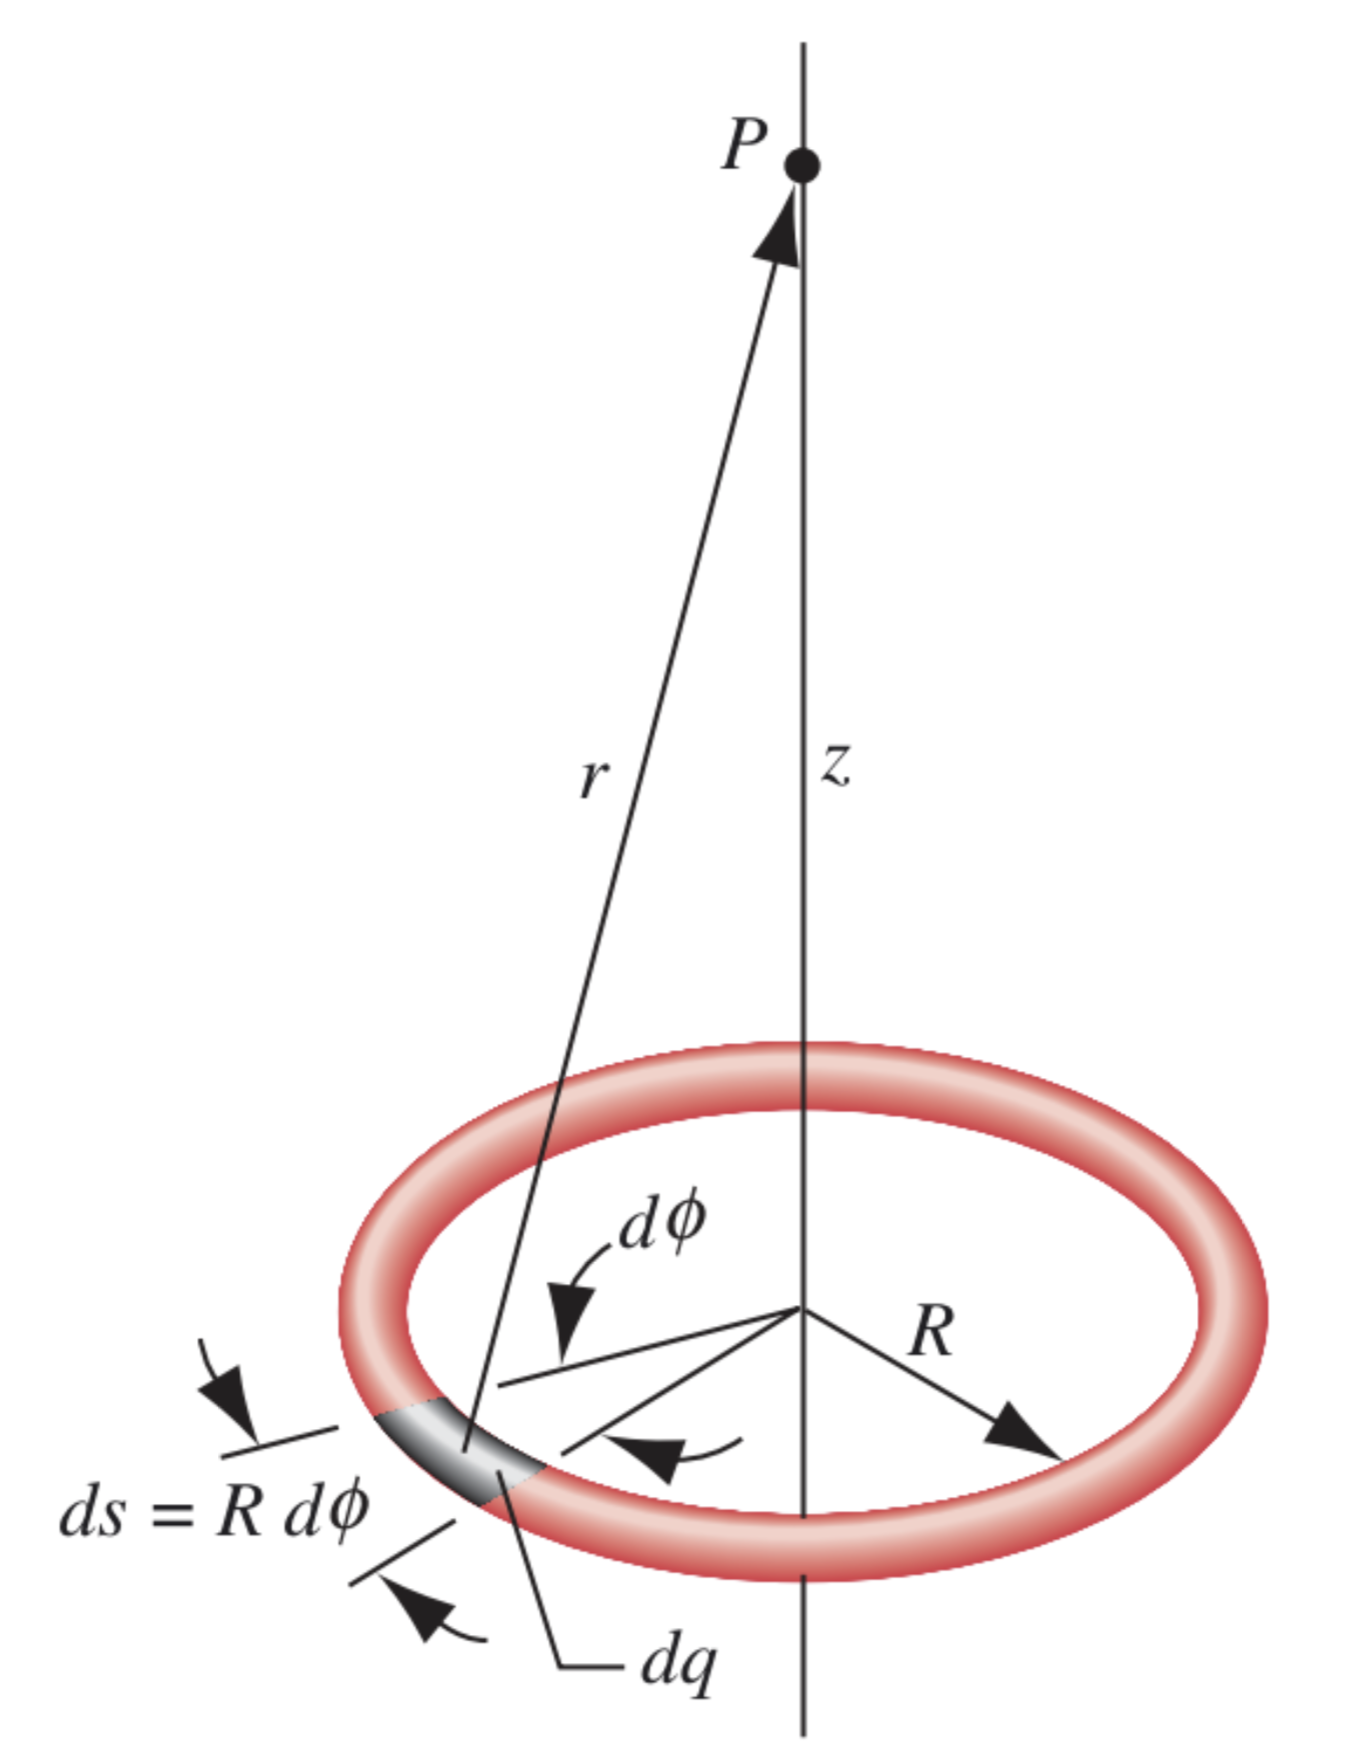
\includegraphics[scale=0.15]{potential}
  \caption{A uniformly charged ring with a potential $P$ and charge element $dq$.}
\end{marginfigure}
%
such that $\| \Phi \| = EA \cos \theta$ where $\theta$ is the angle between the field and field lines. The electric field outside a conductor is given by  \begin{equation}
  E = \frac{\sigma}{\varepsilon_0} \iff q = \iint \sigma \; dA
\end{equation}
The change in electric potential is defined as \begin{equation}
  \Delta U = kq_1q_2 (\Delta r^{-1})
\end{equation}
For a system of charge, the \textbf{potential energy} is \begin{equation}
  U = k \sum_i \sum_{j\neq i} \frac{q_iq_j}{\r}
\end{equation}
Consequently, the change in \textbf{electric potential} is \begin{equation}
  \Delta V = \frac{\Delta U}{q_0} = - \frac{W}{q_0} = - \int \b E \cdot d \b s
\end{equation}

\begin{marginfigure}
  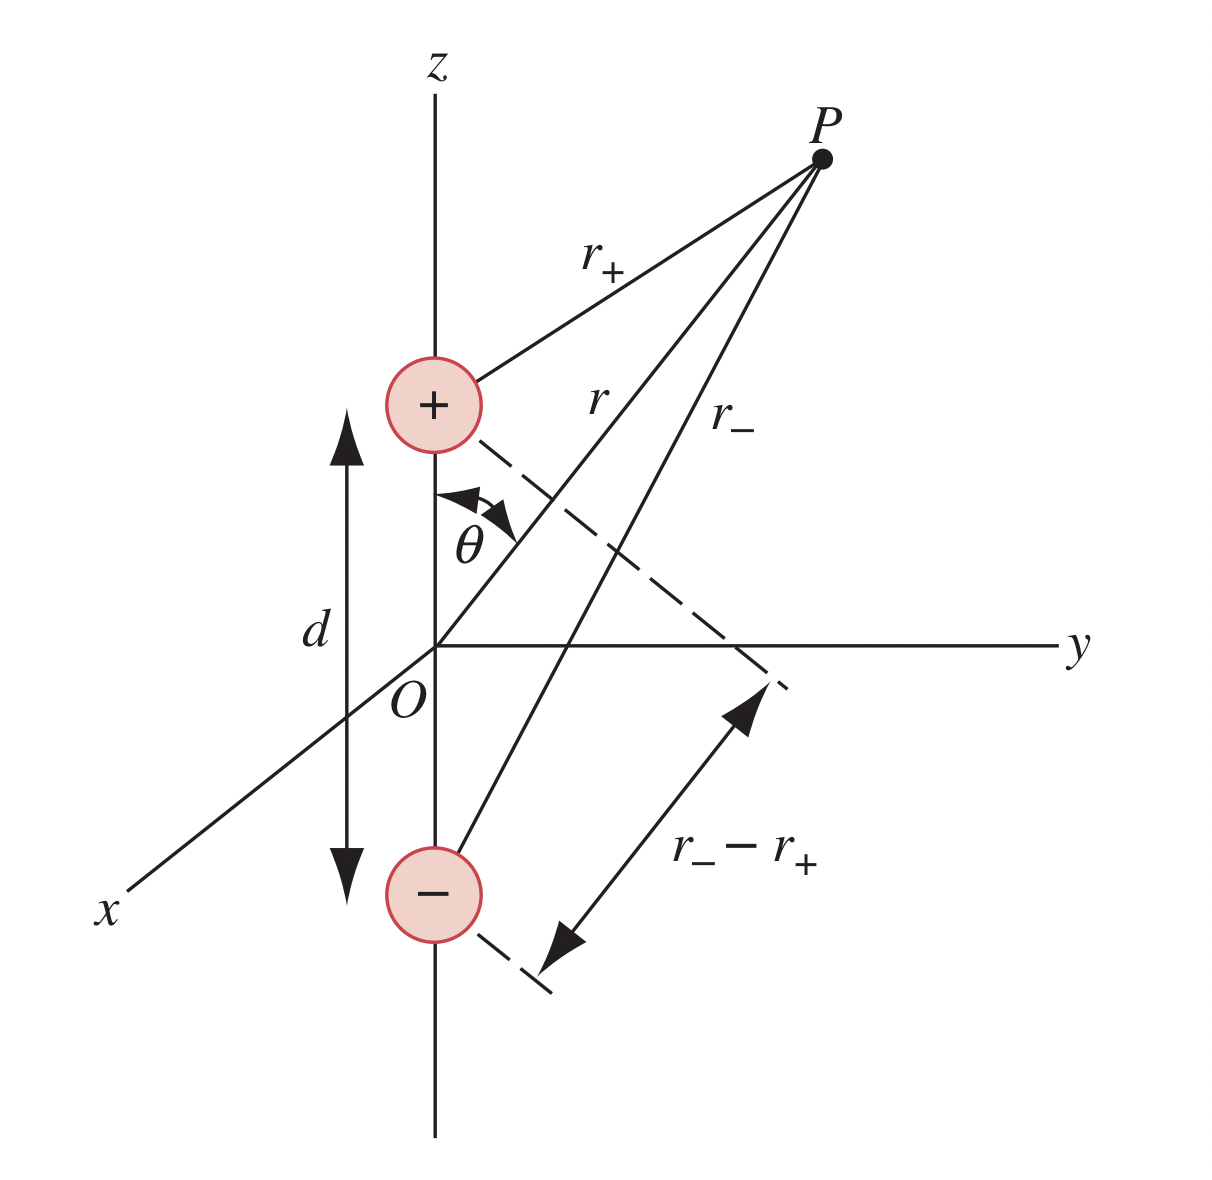
\includegraphics[width=1\textwidth]{dipole2}
  \caption{The geometry for calculating $V$ at $P$ for a dipole.}
\end{marginfigure}

The electric potential at a point is thus defined as \begin{equation}
  V = k \iiint^b_a \frac{dq}{\r} = k \sum \frac{q_i}{\r} \sim k \frac{p \cos \theta}{\r^2}
\end{equation}
where the latter equivalence holds for dipoles. A surface on which the potential has the same value everywhere is \textbf{equipotential} such that $\Delta V = W = 0$. The field lines must everywhere be perpendicular to the equipotential surfaces, which implies all conductors are equipotential.

\chapter{Electrodynamics}

\section{Current}

\textsc{The electric} current is defined as \begin{equation}
  i = \frac{dq}{dt} = \int \b j \cdot d \b A
\end{equation} where $j$ is the current density and is opposite the motion of electrons. The net charge passing through is therefore \begin{equation}
  q = \int i \, dt
\end{equation}
The current density is defined as \begin{equation}
  \b j = q/At = - en \b v = \sigma \b E
\end{equation}
\begin{marginfigure}
  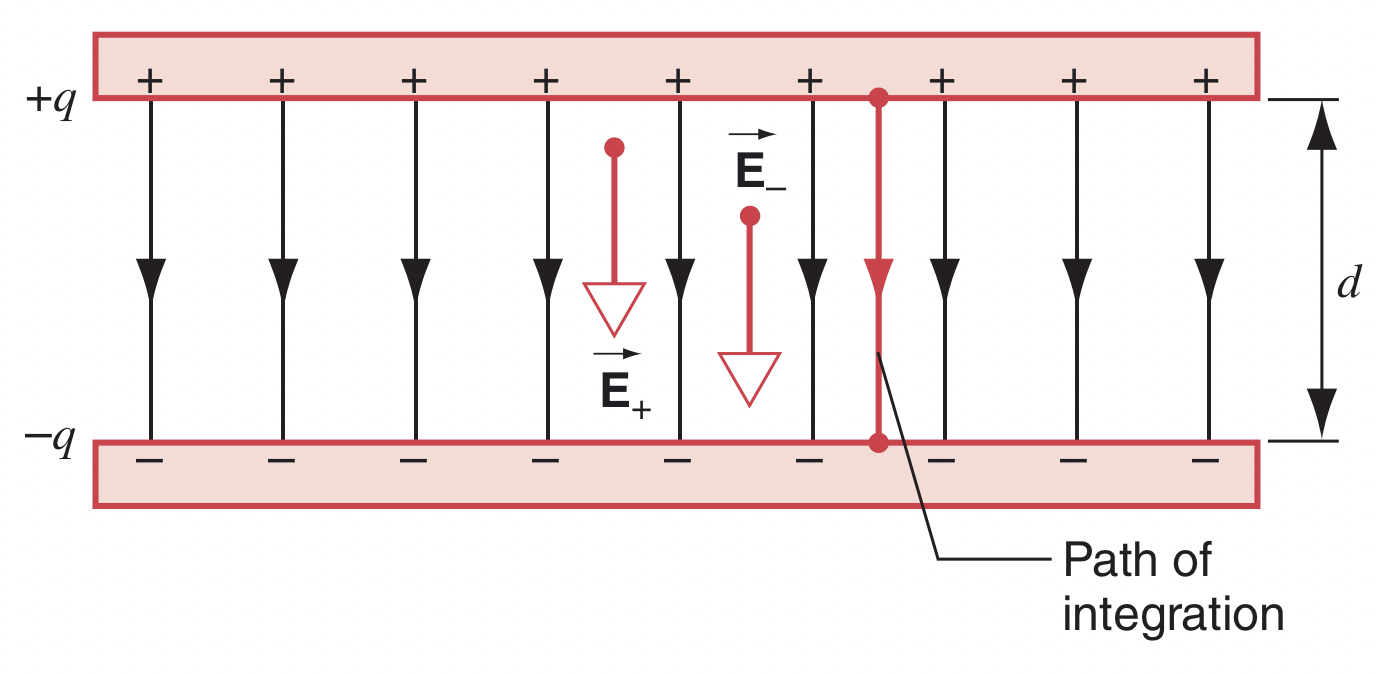
\includegraphics[width=1\textwidth]{ppc}
  \caption{A parallel-plate capacitor.}
\end{marginfigure}
where $n$ is the electron density and $\sigma = q/A$ is the conductivity. Furthermore, the net charge passing through the surface $q = enAL$. The resistance of the material is thus $R = L/\sigma A = \Delta V / i$.

\section{Capacitance}
\textbf{Capacitance} is defined as \begin{equation}
  C = q / \Delta V
\end{equation}
In a PPC, SC, and CC, the potential is derived via \begin{equation}
  \Delta V_{ppc} = \frac{qd}{\epsilon A} \qquad \Delta V_{sc} =kq \left(\frac{1}{a} - \frac{1}{b} \right) \qquad \Delta V_{ss} = \frac{q \ln (b-a)}{2 \pi \epsilon L}
\end{equation}
In a parallel combination of capacitors, \begin{equation}
  q = \sum q  = C_{eq} \Delta V \iff  C_{eq} = \sum C
\end{equation}
and in a series combination, \begin{equation}
  \Delta V = \sum \Delta V = q/C_{eq} \iff C_{eq}^{-1} = \sum C^{-1}
\end{equation}
As well, the potential energy in a capacitor is \begin{equation}
  dU = \Delta V \, dq \iff U = \int_0^q dU = \frac{q^2}{2C}
\end{equation}
with $q = C \Delta V$. Specifically, the energy $U$ is stored in $E$ in the region.


\end{document}
